\documentclass[10pt,a4paper]{scrartcl}
\usepackage[a4paper,vmargin={30mm},hmargin={30mm}]{geometry}
\usepackage[utf8x]{inputenc} % Unicode-Encoding
\usepackage[ngerman]{babel} % Neudeutsche Silbentrennung (mehrsprachiges Dokument)
\usepackage{ucs}
\usepackage{amsmath}
\usepackage{amsfonts}
\usepackage{amssymb}
\usepackage{parskip} % Skip indentation of first row
\usepackage{graphicx} % Graphics support
\usepackage{longtable} % Tables across several pages
\usepackage{hyperref} % Hyperlinks
\author{Danilo Bargen}
\title{Theoriesammlung Analysis 2}

\begin{document}

\begin{titlepage}
	\maketitle
	\vspace{120mm}
	\center\includegraphics{hsr_logo.png}
	\thispagestyle{empty} % Don't start page numbers on this page
\end{titlepage}

\tableofcontents\newpage

\section{Integralrechnung}

\subsection{Definition des Integrals}

Die Definition des Integrals lautet
$$\int\limits_a^b f = \lim_{n \mapsto \infty}\left(\sum_{i=1}^n f(x_i) \cdot \Delta x\right)$$
mit
$$\Delta x = \frac{b-a}{n}$$
und
$$x_i = a + i \cdot \Delta x$$


\subsection{Summenformeln}

$$\sum_{i=1}^n i = \frac{n(n+1)}{2}$$
$$\sum_{i=1}^n i^2 = \frac{n(n+1)(2n+1)}{6}$$
$$\sum_{i=1}^n i^3 = \left(\frac{n(n+1)}{2}\right)^2$$


\subsection{Graphische Interpretation von Integralen}

Wir betrachten das Integral
$$\int\limits_a^b f$$
Wir nennen die Fläche, welche horizontal durch zwei Abszissen und vertikal
durch die Abszissenachse und den Funktionsgraphen begrenzt sind als
\textit{Fläche unter dem Funktionsgraphen}. Es sind nun zwei Fälle zu unterscheiden:

\begin{itemize}
\item Wenn $a < b$ ist:\\
    Dann sind Flächen unter Funktionsgraphen mit positiver Ordinate positiv und
    solche mit negativen Ordinaten negativ zu zählen.
\item Wenn $a > b$ ist:\\
    Dann sind Flächen unter Funktionsgraphen mit positiver
    Ordinate negativ und solche mit negativen Ordinaten positiv zu zählen.
\end{itemize}


\subsection{Vorzeichenregeln und Additivität}

Falls die beteiligten Integrale existieren, gilt
\begin{itemize}
\item Vertauschen der Integralgrenzen ändert das Vorzeichen des Integrals
$$\int\limits_a^b f = - \int\limits_b^a f$$
\item Aneinanderstossende Integrale können zusammengefasst werden.
$$\int\limits_a^b f + \int\limits_b^c f = \int\limits_a^c f$$
\end{itemize}


\subsection{Linearitätsregeln für Integrale}

Seien $f$ und $g$ auf dem intervall $[a;b]$ integrierbare Funktionen und $c$ eine
Konstante. Dann gelten die beiden Linearitätsgesetze:
$$\int\limits_a^b (f + g) = \left(\int\limits_a^b f\right) + 
    \left(\int\limits_a^b g\right)$$
$$\int\limits_a^b (c \cdot f) = c \int\limits_a^b f$$


\subsection{Numerische Berechnung von Integralen}

\subsubsection{Trapezregel}

Die allgemeine Formel für die Trapezregel lautet:

$$\int\limits_a^b f = \left[\frac{f(a) + f(b)}{2} + \sum_{i=1}^{n-1} f(x_i)\right] \Delta x$$
mit
$$\Delta x = \frac{b-a}{n} \textrm{ und } x_i = a + i \cdot \Delta x$$

\subsubsection{Simpson-Regel}

Sei $f$ eine auf $[a;b]$ viermal differenzierbare Funktion und $n$ eine gerade Zahl.
Ferner sei
$$x_i = a + i \cdot \Delta x \textrm{ mit } \Delta x = \frac{b-a}{n}
    \textrm{ und } y_i = f(x_i)$$
Dann ist
$$S_n = \frac{\Delta x}{3}(y_0 + 4y_1 + 2y_2 + 4y_3 + 2y_4 + ... + 4y_{n-1} + y_n)$$
$$= \frac{\Delta x}{3}\left(y_0 + y_n + 4 \sum_{k=1}^{n/2} y_{2k-1} 
    + 2 \sum_{k=1}^{n/2-1} y_{2k}\right)$$
eine Schätzung für das Integral $\int\limits_a^b f$, wobei der Fehler
$$E_n = \left(\int\limits_a^b f\right) - S_n = \frac{b-a}{180}\Delta x^4 f^{(4)}(\xi)
    = \frac{(b-a)^5}{180n^4} f^{(4)}(\xi)$$
$$\textrm{für ein } \xi \in [a;b]$$
beträgt.


\subsection{Integralfunktion}

Gegeben sei eine auf dem Intervall $[a;b]$ integrierbare Funktion $f$. Dann heisst
jede Funktion der Form
$$x \mapsto \int\limits_c^x f$$
für eine Konstante $c \in [a;b]$ eine \textit{Integralfunktion} von $f$.


\subsection{Zusammenhang verschiedener Integralfunktionen}

Verschiedene Integralfunktionen derselben Funktion unterscheiden sich nur durch
eine Konstante. Wenn also
$$\varphi_c := x \mapsto \int\limits_c^x f \textrm{ und } \varphi_d := x \mapsto
    \int\limits_d^x f$$
dann gilt
$$\varphi_d = \varphi_c + k \textrm{ wobei } k \textrm{ konstant}$$



\section{Fouriertransformation}


\subsection{Lineares System}

Ein System $S$ heisst linear, wenn zwei Bedingungen erfüllt sind:
\begin{itemize}
\item Die Antwort einer Summe von Signalen ist gleich der Summe der
Antworten auf die Summanden. Wenn also $x1$ und $x2$ Signale sind, so gilt
$$S(x_1 + x_2) = S(x_1) + S(x_2)$$
\item Die Antwort auf ein mit einer Konstanten multipliziertes
(verstärktes) Signal ist das Produkt dieser Konstante mit der Antwort
des Signals. Wenn also $x$ ein Signal und $c$ eine Konstante ist, dann gilt
$$S(cx) = cS(x)$$
\end{itemize}


\subsection{Zeitinvarianz}

Sei $S$ ein System, $x$ ein beliebiges Eingangssignal und
$$\tilde{x} = t \mapsto x(t - \tau)$$
das um $\tau$ verzögerte Eingangssignal. Dann ist die Antwort auf das verzögerte
Eingangssignal
$$\tilde{y} = S(\tilde{x})$$
Ferner sei
$$y = S(x)$$
die Antwort des Systems auf das Eingangssignal und
$$\hat{y} := t \mapsto y(t-\tau)$$
die verzögerte Antwort auf das Eingangssignal.
Nun heisst $S$ \textit{zeitinvariant}, wenn
$$\tilde{y} = \hat{y}$$


\subsection{Linearkombinationen gleichperiodischer Funktionen}

Linearkombinationen periodischer Funktionen derselben Periode sind
ebenfalls periodisch mit dieser Periode. Oder formal: Seien $f$ und
$g$ zwei Funktionen mit derselben Periode $p$ und $a$ sowie $b$ zwei
Konstanten. Dann ist auch die Funktion
$$af+bg$$
periodisch mit der Periode $p$.


\subsection{Fourier-Entwicklung periodischer Funktionen}

\subsubsection{Sinus-Kosinus-Form}
Wir betrachten ein stückweise stetiges, mit der Grundperiode $T$
periodisches Signal $s$. Dann heisst die Funktion
$$f_n := t \mapsto a_0 + \sum_{k=1}^n \left[ a_k \cos(k\omega_1t) + b_k\sin(k\omega_1t)\right]$$
mit
$$\omega_1 = \frac{2\pi}{T}$$
$$a_0 = \frac{1}{T} \int\limits_0^T s(t) dt$$
$$a_k = \frac{2}{T} \int\limits_0^T s(t) \cos(k\omega_1t) dt$$
$$b_k = \frac{2}{T}\int\limits_0^T s(t) \sin(k\omega_1t) dt$$
für $k \in \{1...n\}$ seine \textit{Fourierentwicklung} der Ordnung $n$.

$\omega_1$ heisst die \textit{Grundkreisfrequenz}, $a_0$ die \textit{Konstante},
$a_k$ und $b_k$ die \textit{Koeffizienten}.

\subsubsection{Spektral-Form}
Neben dieser sogenannten \textit{Sinus-Kosinus-Form} gibt es die für die
Praxis wichtigere \textit{Amplituden-Phasen-Form} oder \textit{Spektral-Form}
$$f_n := t \mapsto A_0 + \sum_{k=1}^n A_k \cos(k\omega_1t - \varphi_k)$$
Die Bestimmungsstücke der Amplituden-Phasen-Form können nicht direkt
berechnet werden, sondern auf dem Umweg über die Koeffizienten
der Sinus-Kosinus-Form. Dabei gilt folgender Zusammenhang:
\begin{itemize}
\item $A_0 = a_0$
\item Ein Punkt in der Ebene, der die kartesischen Koordinaten $(a_k, b_k)$
hat, hat die Polarkoordinaten $(A_k, \varphi_k)$
\end{itemize}


\subsection{Koordinatentransformation Kartesisch / Polar}

Koordinaten aus dem Kartesischen- oder Polarkoordinatensystem können
folgendermassen transformiert werden:

\begin{center}
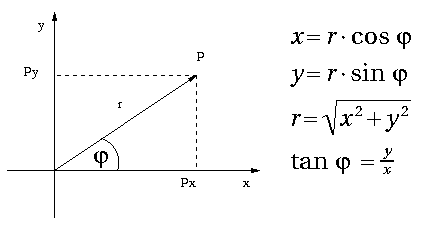
\includegraphics[scale=0.5]{img/Koordinatentransformation.png}
\end{center}

Der Radius $r$ aus dem Polarkoordinatensystem entspricht dabei $A$ in der
Spektralform einer Fourierentwicklung.

Um den Winkel $\varphi$ im Interval $(-\pi, \pi]$ zu berechnen, gibt es mehrere
Möglichkeiten. Mithilfe des Arkustangens:
$$\varphi = \begin{cases}
\arctan\frac{y}{x} & \mathrm{f\ddot ur}\ x > 0\\
\arctan\frac{y}{x} + \pi & \mathrm{f\ddot ur}\ x < 0,\ y \geq 0\\
\arctan\frac{y}{x} - \pi & \mathrm{f\ddot ur}\ x < 0,\ y < 0\\
+\pi/2 & \mathrm{f\ddot ur}\ x = 0,\ y > 0\\
-\pi/2 & \mathrm{f\ddot ur}\ x = 0,\ y < 0\\
\end{cases}$$

Oder alternativ mithilfe des Arkuskosinus:
$$\varphi = \begin{cases}
+\arccos\frac{x}{r} & \mathrm{f\ddot ur}\ y\geq 0\\
-\arccos\frac{x}{r} & \mathrm{f\ddot ur}\ y<0
\end{cases}$$


\subsection{Fourierreihen}

Die Funktion
$$f := t \mapsto a_0 + \sum_{k=1}^{\infty} \left[a_k \cos(k\omega_1t) + b_k \sin(k\omega_1t)\right]$$
$$= t \mapsto A_0 + \sum_{k=1}^{\infty} A_k \cos(k\omega_1 t - \varphi_k)$$
heisst die \textit{Fourierreihe} von $s$.


\subsection{Kriterium von Dirichlet}

Sei $s$ ein mit $T$ periodisches Signal, das innerhalb einer Periode aus
endlich vielen stetigen Stücken zusammengesetzt ist. Dann konvergieren die
Werte der Fourierreihe $f$ und zwar
\begin{itemize}
\item an Stellen $t$, an denen das Signal stetig ist, gegen den Signalwert
$$f(t) = s(t)$$
\item an Stellen $t$, an denen das Signal nicht stetig ist, gegen den Mittelwert der beiden einseitigen Grenzwerte
$$f(t) = \frac{\lim\limits_{\tau \mapsto t-}(f(\tau)) + \lim\limits_{\tau \mapsto t+}(f(\tau))}{2}$$
\end{itemize}


\subsection{Fourierreihen gerader und ungerader Signale}

Ein gerades, mit der Periode $T$ periodisches Signal $g$ besitzt eine reine
Kosinusreihe
$$f_g := t \mapsto a_0 + \sum_{k=1}^{\infty} \left[ a_k \cos(k\omega_1t)\right] \textrm{ mit } \omega_1 = \frac{2\pi}{T}$$
wobei
$$a_k = \frac{4}{T} \int\limits_0^{T/2} g(t) \cos(k\omega_1t) dt$$
gilt.

Ein ungerades, mit der Periode $T$ periodisches Signal $u$ besitzt eine reine
Sinusreihe
$$f_u := t \mapsto \sum_{k=1}^{\infty} \left[ b_k \sin(k\omega_1t)\right] \textrm{ mit } \omega_1 = \frac{2\pi}{T}$$
wobei
$$b_k = \frac{4}{T} \int\limits_0^{T/2} u(t) \sin(k\omega_1t) dt$$
gilt.


\subsection{Linearität der Fourierkoeffizienten}

$s_1$ und $s_2$ seien zwei Signale mit derselben Periode $T$. Die Konstanten
ihrer Fourierreihen seien $a_{1,0}$ beziehungsweise $a_{2,0}$ und die
Koeffizienten $a_{1,k}$, $b_{1,k}$ beziehungsweise $a_{2,k}$, $b_{2,k}$.

Dann ist die Summe beiden Signale
$$s = s_1 + s_2$$
periodisch mit derselben Periode und für die Konstante $a_0$, sowie die
Koeffizienten $a_k$ und $b_k$ ihrer Fourierreihe gelten folgende Beziehungen:
$$a_0 = a_{1,0} + a_{2,0}$$
$$a_k = a_{1,k} + a_{2,k}$$
$$b_0 = b_{1,k} + b_{2,k}$$
Ist ferner $c$ eine Konstante, so hat auch das Signal
$$\tilde{s} = c \cdot s$$
dieselbe Periode $T$, und die Konstante und Koeffizienten der
Fourierentwicklung sind
$$\tilde{a_0} = c \cdot a_0$$
$$\tilde{a_k} = c \cdot a_k$$
$$\tilde{b_x} = c \cdot b_k$$

\vspace{120mm}
Stand Dokument: Bis und mit Kapitel 4.2.3


\section{Differentialgleichungen}

...

\end{document}
